% Part of main.tex; compile main.tex.
\subsection{Results}
\label{sec:results}

In this section, we present our measurements. We first characterize the I/O
cost of each backend without computation. We then answer RQ1 to RQ4, and
lastly we examine how sensitive the results are to the compute-to-I/O ratio
and to the output size.

\subsubsection{I/O-only baselines}
\label{sec:io0}
% Generated by src/analysis/plots_measured.py; do not edit.
\begin{table}[t]
\centering
\small
\setlength{\tabcolsep}{3.5pt}
\begin{tabular}{@{}l r r r r r@{}}
\toprule
Backend & GiB/step & Sync (s) & Async (s) & Async/sync & Sync GB/s \\
\midrule
POSIX & 0.75 & 0.07 & 0.08 & 1.06 & 10.9 \\
 & 3 & 0.29 & 0.26 & 0.89 & 10.9 \\
 & 12 & 1.26 & 1.77 & 1.41 & 10.3 \\
 & 48 & 8.23 & 4.28 & 0.52 & 6.3 \\
\addlinespace[2pt]
MPI-IO & 0.75 & 0.44 & 0.79 & 1.80 & 1.8 \\
 & 3 & 1.77 & 3.65 & 2.06 & 1.8 \\
 & 12 & 8.69 & 16.25 & 1.87 & 1.5 \\
 & 48 & 36.87 & 68.85 & 1.87 & 1.4 \\
\addlinespace[2pt]
HDF5 & 0.75 & 0.38 & 0.42 & 1.10 & 2.1 \\
 & 3 & 2.40 & 1.80 & 0.75 & 1.3 \\
 & 12 & 10.69 & 5.84 & 0.55 & 1.2 \\
 & 48 & 45.54 & 30.43 & 0.67 & 1.1 \\
\addlinespace[2pt]
ADIOS2 & 0.75 & 0.08 & 0.10 & 1.24 & 9.8 \\
 & 3 & 0.37 & 0.32 & 0.87 & 8.7 \\
 & 12 & 1.85 & 2.61 & 1.40 & 6.9 \\
 & 48 & 7.99 & 8.25 & 1.03 & 6.5 \\
\bottomrule
\end{tabular}
\caption{Measured I/O-only time per step (48 ranks, 5 steps, no computation; mean of the repetitions). Async/sync below 1 means the asynchronous mode is faster even without computation to overlap.}
\label{tab:io0}
\end{table}

Before adding computation, we measure each backend writing 5 timesteps with
no compute phase at all. Table~\ref{tab:io0} shows the results for 48 ranks,
with \IonPosixMd runs per configuration. These runs determine the I/O cost
that the compute surrogates later try to hide, and they show that the
backends differ by an order of magnitude.

\paragraph{Cache-absorbed and write-back regimes.} At 0.75\,GiB per step,
POSIX and ADIOS2 write \IobwPosixXs and \IobwAdiosXs\,GB/s, respectively. This
is memory speed, because the whole run fits in the page cache. At 48\,GiB
per step (240\,GiB per run), their bandwidth drops to \IobwPosixLg and
\IobwAdiosLg\,GB/s, which is the rate at which the RAID array absorbs
write-back. With 10 instead of 5 steps at 12\,GiB per step, POSIX sustains
only about 1.6 to 2.0\,GB/s in our spot checks, because a larger fraction of
each run waits for write-back. For this reason, every later experiment
measures its own I/O-only baseline with the same size and number of steps
(\srcIoBaseline) instead of reusing these numbers.

\paragraph{Collective I/O limits MPI-IO and HDF5.} MPI-IO and HDF5 both write
through the collective buffering of ROMIO with 8 aggregators. They reach only
\IobwMpiioMd and \IobwHdfMd\,GB/s at 12\,GiB per step, which is roughly a
seventh of the bandwidth of POSIX at the same size. In addition, HDF5 has the
largest fixed cost per step, \IosyncHdfXs\,s at 0.75\,GiB compared to
\IosyncPosixXs\,s for POSIX. This cost is dominated by the collective
creation of datasets and by metadata operations.

\paragraph{Asynchronous mode without computation.} With nothing to overlap,
an ideal asynchronous mode would match the synchronous one. However, POSIX
AIO and the HDF5 asynchronous VOL are faster at large sizes, with an
async/sync ratio of \IoratioPosixLg and \IoratioHdfMd, respectively, because
the write of one step overlaps the buffer copy and setup of the next. The
ratio of ADIOS2 ranges from \IoratioAdiosSm to \IoratioAdiosMd. In contrast,
non-blocking MPI-IO is \IoratioMpiioXs to \IoratioMpiioSm$\times$
\emph{slower} than blocking MPI-IO at every size. This is consistent with
contention between the asynchronous progress thread of MPICH and the
application thread, which share a hardware thread under our default
binding. The core-allocation experiment in Section~\ref{sec:rq4} supports
this explanation.

\subsubsection{Run time compared to the sleep prediction (RQ1)}
\label{sec:rq1}
\begin{figure}[t]
\centering
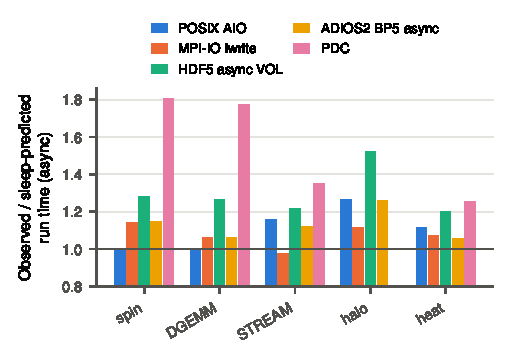
\includegraphics[width=\columnwidth]{figures/m_excess.pdf}
\caption{Observed run time of the asynchronous run with each compute
surrogate, divided by the run time that the \texttt{sleep} run predicts for
the same compute length (120\,GiB per run, 48 ranks; PDC: 47 clients and 1
server). Values above 1 mean the application runs longer than a
\texttt{sleep}-based evaluation predicts. PDC has no halo result, because
its asynchronous halo run did not complete.}
\label{fig:excess}
\end{figure}

\begin{figure}[t]
\centering
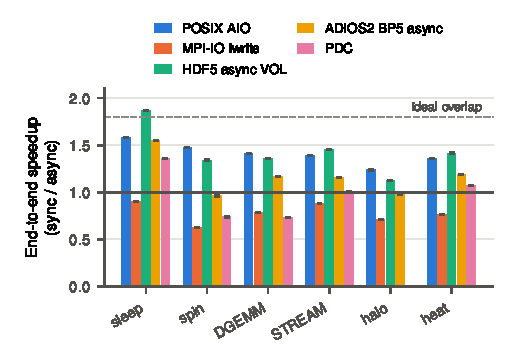
\includegraphics[width=\columnwidth]{figures/m_speedup.pdf}
\caption{End-to-end speedup of asynchronous over synchronous I/O for each
compute surrogate (same runs as Fig.~\ref{fig:excess}). The dashed line is
the ideal $(t_{comp}+t_{io})/\max(t_{comp},t_{io})$ for
$t_{comp}=1.25\,t_{io}$.}
\label{fig:speedup}
\end{figure}

In Fig.~\ref{fig:excess}, we compare the observed run time of each
asynchronous run with the run time that the \texttt{sleep} run predicts for
the same compute length (Section~\ref{sec:metrics}). In \ExcLongerFive of
the \ExcN configurations, the application runs at least 5\% longer than
\texttt{sleep} predicts, and up to \ExcMaxPct\% longer. The effect is largest
for PDC, which runs \ExcminpctPdc\% to \ExcmaxpctPdc\% longer with every
working surrogate, even though its server runs on a reserved core
(Section~\ref{sec:rq4}). Among the backends whose engine runs inside the
application, the effect is largest for the HDF5 asynchronous VOL, which runs \ExcminpctHdf\% to
\ExcmaxpctHdf\% longer with every working surrogate. ADIOS2 runs
\ExcminpctAdios\% to \ExcmaxpctAdios\% longer, and MPI-IO up to
\ExcmaxpctMpiio\% longer. POSIX AIO is the least affected. With spin and
DGEMM, its run time matches the \texttt{sleep} prediction, while with STREAM,
heat, and halo it runs \ExcpctPosixStream\%, \ExcpctPosixHeat\%, and
\ExcpctPosixHalo\% longer. It is important to note that each configuration
was run once, so differences of a few percent are within the run-to-run
variation of this node (Section~\ref{sec:workload}).

Fig.~\ref{fig:speedup} shows the same runs as end-to-end speedups, which is
the metric most prior work reports. For the three backends where
asynchronous I/O helps, \texttt{sleep} yields the largest speedup of all
surrogates: \SpPosixSleep$\times$ for POSIX AIO, \SpHdfSleep$\times$ for the
HDF5 asynchronous VOL, and \SpAdiosSleep$\times$ for ADIOS2. Every surrogate
that performs work lowers this benefit. The speedup of POSIX ranges from
\SpPosixSpin$\times$ with spin to \SpPosixHalo$\times$ with halo, the speedup
of HDF5 from \SpHdfStream$\times$ to \SpHdfHalo$\times$, and the speedup of
ADIOS2 from \SpAdiosHeat$\times$ to \SpAdiosSpin$\times$. In addition,
MPI-IO is slower than its blocking mode in every configuration, from
\SpMpiioSleep$\times$ with \texttt{sleep} to \SpMpiioSpin$\times$ with spin.
However, speedups divide two separate runs, and they inherit the
variation of the synchronous run. In our main experiment, the synchronous
run with \texttt{sleep} had the slowest synchronous I/O of all surrogates
for every backend (Section~\ref{sec:threats}). This inflates the
\texttt{sleep} speedups, which is why we base RQ1 on the comparison of
asynchronous run times in Fig.~\ref{fig:excess}.

\subsubsection{Where the cost appears (RQ2)}
\label{sec:rq2}
\begin{figure*}[t]
\centering
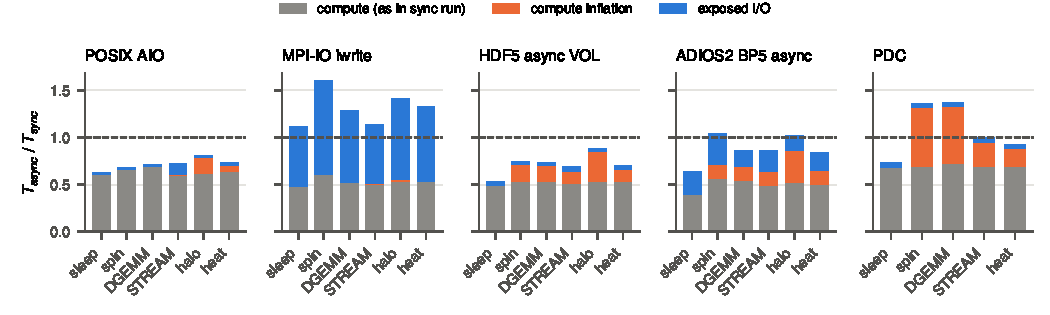
\includegraphics[width=\textwidth]{figures/m_decomp.pdf}
\caption{Breakdown of the time of an asynchronous run, relative to the
synchronous run with the same surrogate. The dashed line marks the
synchronous run time, and values below 1 mean that asynchronous I/O helps. Gray: compute time as in the synchronous run.
Orange: compute inflation caused by background I/O. Blue: exposed I/O. PDC
has no halo result.}
\label{fig:decomp}
\end{figure*}

\begin{figure*}[t]
\centering
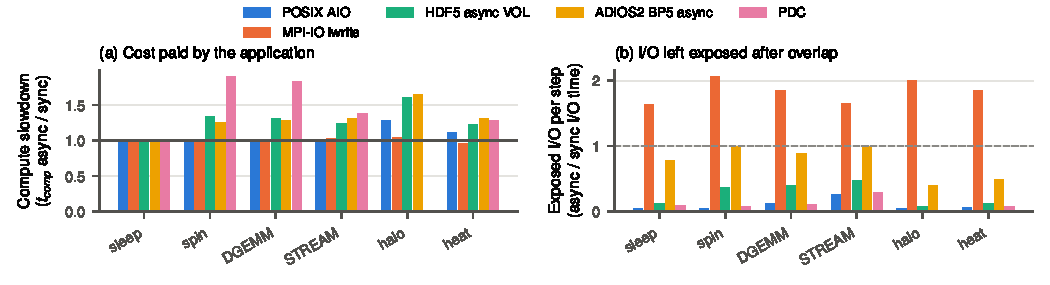
\includegraphics[width=\textwidth]{figures/m_breakdown.pdf}
\caption{(a)~Slowdown of the compute phase of the asynchronous run relative
to the synchronous run. (b)~I/O still exposed per step in the asynchronous
run, relative to the synchronous I/O time per step (dashed line: no hiding
at all).}
\label{fig:breakdown}
\end{figure*}

In Figs.~\ref{fig:decomp} and~\ref{fig:breakdown}, we attribute the lost
benefit to the compute side or to the I/O side. The backends fall into two
groups.

\paragraph{Compute-side interference (POSIX, HDF5, ADIOS2, and PDC).} For these
backends, little I/O remains exposed, and the loss appears as a longer
compute phase. The size of the effect depends on the design of the
background engine:
\begin{itemize}
  \item \textbf{POSIX AIO} is the least intrusive. Spin, DGEMM, and STREAM
        slow down by at most 2\%, which is consistent with its single glibc
        helper thread spending most of its time blocked on write-back rather
        than running. Only the communicating surrogates are affected, with a
        slowdown of \SlowPosixHalo$\times$ for halo and
        \SlowPosixHeat$\times$ for heat.
  \item \textbf{The HDF5 asynchronous VOL} slows down \emph{every} working
        surrogate, from \SlowHdfHeat$\times$ for heat to
        \SlowHdfHalo$\times$ for halo. This includes the spin loop, which
        only uses the arithmetic units (\SlowHdfSpin$\times$). The Argobots
        thread executes HDF5 operations on the hardware thread of the rank
        and competes for it directly.
  \item \textbf{ADIOS2 BP5} in Guided mode behaves similarly, with a
        slowdown of \SlowAdiosSpin$\times$ for spin and \SlowAdiosHalo$\times$
        for halo. In this mode, ADIOS2 deliberately writes during the
        computation blocks announced by the application, which is exactly
        when the computation needs the core.
  \item \textbf{PDC} slows down every working surrogate the most, from
        \SlowPdcHeat$\times$ for heat to \SlowPdcSpin$\times$ for spin,
        although its server runs on a separate core. The cause is on the
        client side: the progress thread of each client rank polls the
        network on the hardware thread of the rank. As a result, the
        speedup with spin and DGEMM drops below 1 (\SpPdcSpin$\times$ and
        \SpPdcDgemm$\times$), compared to \SpPdcSleep$\times$ with
        \texttt{sleep}.
\end{itemize}
For POSIX, HDF5, and ADIOS2, the halo exchange is the most sensitive surrogate.
Therefore, contention reaches the application through MPI and shared-memory
traffic as well as through the CPU.

\paragraph{I/O-side interference (MPI-IO).} With non-blocking collective
MPI-IO, the compute phase is undisturbed, with a slowdown between
\SlowMpiioHeat and \SlowMpiioHalo. However, the background write barely
advances while the application computes. The application then waits for
it at the next step, and the exposed I/O per step exceeds the synchronous
I/O time (Fig.~\ref{fig:breakdown}b). Over the run, the exposed I/O is
\DcexposecMpiioSleep\,s with \texttt{sleep} and \DcexposecMpiioSpin\,s with
spin.

In both groups, the run time that the application observes is longer than a
\texttt{sleep}-based evaluation predicts. A study that reports only the
observed I/O time would see the POSIX and HDF5 results as nearly complete
hiding (Fig.~\ref{fig:breakdown}b) and would miss the inflated compute phase
entirely.

\summarybox{With real computation, the application runs longer than a
\texttt{sleep}-based evaluation predicts in \ExcLongerFive of \ExcN
configurations, by up to \ExcMaxPct\%. For POSIX AIO, the HDF5 asynchronous
VOL, and ADIOS2, the cost appears as a slower computation, and the halo
exchange is the most sensitive surrogate. For non-blocking MPI-IO, the
computation is undisturbed, but the I/O does not progress during it and is
exposed later.}

\subsubsection{Sleep-based estimates and a mini-application (RQ3)}
\label{sec:rq3}
% Generated by src/analysis/plots_measured.py; do not edit.
\begin{table}[t]
\centering
\small
\setlength{\tabcolsep}{2.2pt}
\begin{tabular}{@{}l c c c c c c@{}}
\toprule
 & & \multicolumn{3}{c}{Speedup} & \multicolumn{2}{c}{Longer than sleep predicts} \\
\cmidrule(lr){3-5}\cmidrule(l){6-7}
Backend & $t_{comp}/t_{io}$ & Model & Sleep & Heat & Heat & Worst \\
\midrule
POSIX & 1.72 & 1.58 & 1.58 & 1.36 & +12\% & +26\% (halo) \\
MPI-IO & 1.12 & 1.89 & 0.90 & 0.77 & +7\% & +14\% (spin) \\
HDF5 & 1.10 & 1.91 & 1.87 & 1.42 & +20\% & +52\% (halo) \\
ADIOS2 & 0.99 & 1.99 & 1.55 & 1.19 & +5\% & +26\% (halo) \\
PDC & 2.28 & 1.44 & 1.36 & 1.08 & +26\% & +81\% (spin) \\
\bottomrule
\end{tabular}
\caption{Speedup predicted by the overlap model of Ravi et al.~\cite{ravi2023evaluating} for each backend's measured ratio $t_{comp}/t_{io}$ (no overhead), and measured with \texttt{sleep} and with the heat mini-app. The last two columns give how much longer the asynchronous run with the heat mini-app, and with the least favourable surrogate, takes than the \texttt{sleep} run predicts for the same compute length (Section~\ref{sec:metrics}).}
\label{tab:rq3}
\end{table}

In Table~\ref{tab:rq3}, we compare the benefit predicted by the analytical
model of Ravi et al.\ and by \texttt{sleep} with the benefit that the heat
mini-app obtains. The heat mini-app is the closest stand-in for a real
simulation in our set. The model is evaluated for the measured
compute-to-I/O ratio of each backend, which ranges from \RatioeffAdios for
ADIOS2 to \RatioeffPosix for POSIX. For POSIX and HDF5, the \texttt{sleep}
speedup is close to the model (\SpPosixSleep versus \ModelPosix, and
\SpHdfSleep versus \ModelHdf). This means that a \texttt{sleep}-based
evaluation mostly validates the model against itself. In contrast, the heat
mini-app obtains a lower speedup with every backend, and its asynchronous run
takes \ExcpctPosixHeat\% (POSIX), \ExcpctMpiioHeat\% (MPI-IO),
\ExcpctHdfHeat\% (HDF5), and \ExcpctAdiosHeat\% (ADIOS2) longer than the
\texttt{sleep} run predicts. The least favourable surrogate raises this gap
to up to \ExcmaxpctHdf\%. This mirrors, at kernel scale, the gap between the
4.5 to 4.9$\times$ I/O-time speedups reported with
\texttt{sleep}~\cite{tang2022async} and the 1.5$\times$ end-to-end speedup
observed in Flash-X~\cite{jain2022flashx}.

\subsubsection{Sensitivity to the compute-to-I/O ratio}
\label{sec:sweep}
\begin{figure*}[t]
\centering
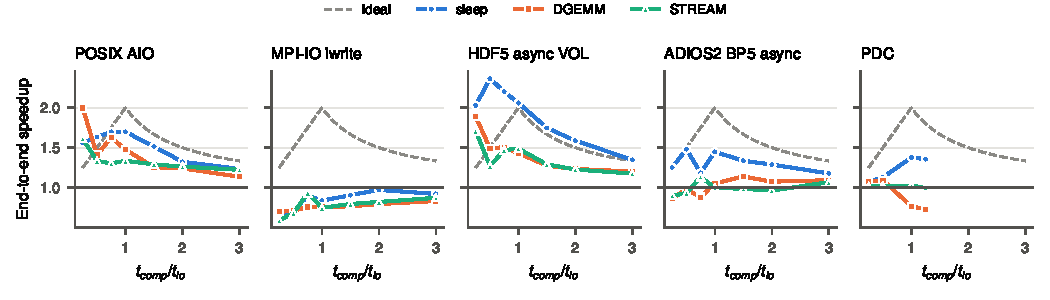
\includegraphics[width=\textwidth]{figures/m_sweep.pdf}
\caption{End-to-end speedup as a function of $t_{comp}/t_{io}$ (12\,GiB per
step, 10 steps), where $t_{io}$ is the synchronous I/O time per step of the
same configuration. The dashed line is the ideal $(r+1)/\max(r,1)$. PDC
(47 clients and 1 server) is measured from 0.25 to 1.25 only.}
\label{fig:sweep}
\end{figure*}

Sleep-based studies choose $t_{comp}$ so that it just covers the I/O. A
single ratio could therefore favor or penalize either kind of surrogate. For
this reason, we sweep $t_{comp}/t_{io}$ from 0.25 to 3 (\srcPhaseSweep), as
shown in Fig.~\ref{fig:sweep}. In the regime used by prior work
($t_{comp}\ge t_{io}$), \texttt{sleep} exceeds DGEMM and STREAM at every ratio
for POSIX, HDF5, and ADIOS2. On average, the \texttt{sleep} speedup is higher
by \SweepgapPosixDgemm\% and \SweepgapPosixStream\% for POSIX,
\SweepgapHdfDgemm\% and \SweepgapHdfStream\% for HDF5, and
\SweepgapAdiosDgemm\% and \SweepgapAdiosStream\% for ADIOS2. For ADIOS2, the
speedup with DGEMM and STREAM stays near 1$\times$ across the whole range,
so no choice of compute length recovers the benefit that \texttt{sleep}
shows. MPI-IO stays below 1$\times$ everywhere and approaches break-even only
for \texttt{sleep} at the largest ratios. Therefore, the gap between
\texttt{sleep} and working surrogates is not an artifact of the ratio used
in the main experiment. At small ratios, the curves are noisier because the
runs are short, and HDF5 and POSIX can exceed the ideal, because their
asynchronous modes also pipeline consecutive writes (Table~\ref{tab:io0}).

For PDC, we measure the ratios 0.25, 0.5, and 1 (\srcPhasePdcSweep) and take
the point at 1.25 from the main experiment. Each PDC run writes 120\,GiB
through a single server, and ratios above 1.25 would take more than
10 minutes per run. The PDC curves show how the cost of the interference
depends on the ratio. The compute slowdown with DGEMM stays at about
\PdcslowDgemm$\times$ at every ratio, but its effect on the run time does
not. At 0.25 and 0.5, the compute phase is shorter than the I/O even when it
is slowed down, so the slowdown is hidden behind the I/O. In this case, DGEMM
reaches its best speedup of \PeakPdcDgemm$\times$ at a ratio of
\PeakatPdcDgemm, close to the \texttt{sleep} speedup at the same ratio. Once the slowed
compute phase is longer than the I/O, it lies on the critical path, and the
speedup with DGEMM drops below 1$\times$, while \texttt{sleep} reaches its
peak of \PeakPdcSleep$\times$ at a ratio of \PeakatPdcSleep. At ratios of 1
and 1.25, the \texttt{sleep} speedup is higher than the speedup with DGEMM
by \SweepgapPdcDgemm\% and higher than with STREAM by \SweepgapPdcStream\%,
and STREAM never exceeds \PeakPdcStream$\times$. Therefore, for PDC, the
regime that \texttt{sleep}-based studies choose, where the computation covers
the I/O, is exactly the regime in which the interference becomes visible in
the run time.

\subsubsection{Effect of output size}
\label{sec:size}
\begin{figure*}[t]
\centering
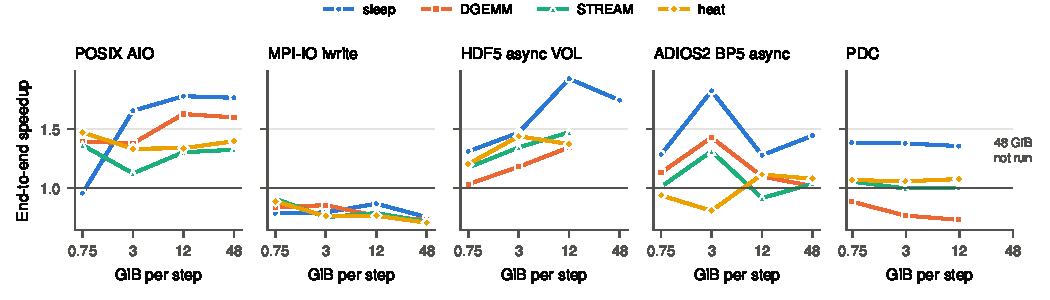
\includegraphics[width=\textwidth]{figures/m_size.pdf}
\caption{End-to-end speedup as a function of the output size per step (48
ranks, 10 steps, and $t_{comp}=1.25\,t_{io}$ for each size). The 48\,GiB
point (480\,GiB per run) is measured for POSIX and ADIOS2 only. PDC uses
47 clients, so its sizes are 0.73, 2.9, and 11.75\,GiB per step.}
\label{fig:size}
\end{figure*}

In Fig.~\ref{fig:size}, we vary the output per step from 0.75\,GiB
(7.5\,GiB per run) to 12\,GiB (120\,GiB per run), as defined in
\srcPhaseSize. At 0.75\,GiB, the output fits in the page cache, the I/O and
compute phases are short, and the results are noisy. In this case, POSIX AIO
is even slower than its blocking mode with \texttt{sleep}
(\SizePosixSleepXs$\times$). Once the I/O is substantial, the speedup with
\texttt{sleep} increases with the size. For POSIX, it increases from
\SizePosixSleepSm$\times$ at 3\,GiB to \SizePosixSleepMd$\times$ at 12\,GiB,
and for HDF5 from \SizeHdfSleepSm$\times$ to \SizeHdfSleepMd$\times$.
However, the working surrogates do not keep pace. At 12\,GiB, the heat
mini-app reaches \SizePosixHeatMd$\times$ with POSIX and
\SizeHdfHeatMd$\times$ with HDF5. For HDF5, the gap between \texttt{sleep} and the
heat mini-app grows with the output size, while for POSIX it is present
from 3\,GiB on. ADIOS2 varies without a clear trend, and MPI-IO stays below
1$\times$ at every size.

At the largest size, 48\,GiB per step (480\,GiB per run), which we measured
for POSIX and ADIOS2, the gap persists. For POSIX, \texttt{sleep} reaches
\SizePosixSleepLg$\times$, while DGEMM, STREAM, and the heat mini-app reach
\SizePosixDgemmLg, \SizePosixStreamLg, and \SizePosixHeatLg$\times$. For
ADIOS2, \texttt{sleep} reaches \SizeAdiosSleepLg$\times$, while the working
surrogates reach only \SizeAdiosDgemmLg to \SizeAdiosHeatLg$\times$, so
asynchronous I/O provides almost no benefit to them. Therefore, the
overstatement of \texttt{sleep} does not disappear when the I/O dominates
the run time.

PDC (\srcPhasePdcSize) shows the most consistent picture of all backends.
The speedup with \texttt{sleep} is nearly constant, from
\SizePdcSleepXs$\times$ at 0.73\,GiB to \SizePdcSleepMd$\times$ at
11.75\,GiB, which is consistent with a single server performing all writes
at a similar rate for every size. The working surrogates stay well below it at every size,
including the smallest one, where the other backends are noisy. STREAM
reaches at most \SizePdcStreamXs$\times$, and the heat mini-app at most
\SizePdcHeatMd$\times$. With DGEMM,
the asynchronous run is slower than the synchronous run at every size, and
the speedup falls from \SizePdcDgemmXs$\times$ to \SizePdcDgemmSm$\times$
and \SizePdcDgemmMd$\times$ as the size grows. We did not run PDC at 47\,GiB
per step, because a single run would take about 90 minutes through one
server.

\summarybox{The advantage of \texttt{sleep} over working surrogates persists
across compute-to-I/O ratios from 0.25 to 3 and across output sizes up to
480\,GiB per run. For HDF5, it grows with the output size. For PDC, it is
present at every size we measured, and it appears as soon as the computation
is long enough to cover the I/O, which is the regime that
\texttt{sleep}-based evaluations target.}

\subsubsection{Core allocation (RQ4)}
\label{sec:rq4}
\begin{figure*}[t]
\centering
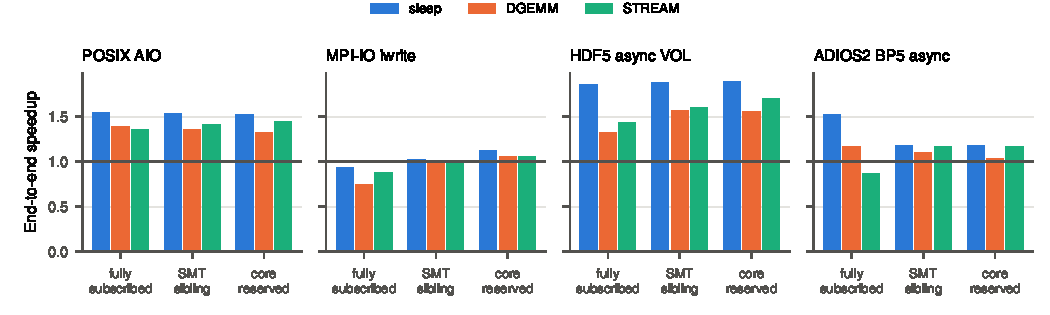
\includegraphics[width=\textwidth]{figures/m_bind.pdf}
\caption{End-to-end speedup under three process placements (12\,GiB per
step): one hardware thread per rank shared with the background engine (fully
subscribed), both hardware threads of the core (SMT sibling), and two
physical cores per rank with 24 ranks (core reserved).}
\label{fig:bind}
\end{figure*}

In Fig.~\ref{fig:bind}, we vary where the background engine can run
(\srcPhaseBind, with the bindings in \srcBinding). Sleep cannot respond to
this choice, because a sleeping thread leaves its core idle anyway. In
contrast, the working surrogates are affected by the placement:
\begin{itemize}
  \item \textbf{HDF5.} Giving the Argobots thread a second hardware thread
        raises the speedup with DGEMM from \BindHdfDgemmFull$\times$ (fully
        subscribed) to \BindHdfDgemmSmt$\times$ (SMT sibling) and
        \BindHdfDgemmReserved$\times$ (core reserved), and the speedup with
        STREAM from \BindHdfStreamFull$\times$ to
        \BindHdfStreamReserved$\times$. The compute slowdown with DGEMM falls
        from \BindslowHdfDgemmFull to \BindslowHdfDgemmReserved accordingly.
        However, the gap to \texttt{sleep} (\BindHdfSleepReserved$\times$)
        remains.
  \item \textbf{MPI-IO.} Reserving a core turns the loss into a small gain.
        The speedup with \texttt{sleep} rises from \BindMpiioSleepFull$\times$
        to \BindMpiioSleepReserved$\times$, and with DGEMM from
        \BindMpiioDgemmFull$\times$ to \BindMpiioDgemmReserved$\times$. This
        supports the explanation that the progress thread, starved of CPU
        time when it shares the hardware thread of the rank, stalls
        non-blocking MPI-IO.
  \item \textbf{POSIX AIO} is largely insensitive to the three pinned
        placements, as expected from its low CPU demand.
  \item \textbf{ADIOS2} shows no consistent gain from extra hardware
        threads, and its \texttt{sleep} speedup is highest when fully
        subscribed. With a single run per configuration, we cannot tell
        whether this reflects a different aggregation behavior of ADIOS2
        under other placements or run-to-run variation.
  \item \textbf{PDC.} The server of PDC already runs on a reserved core,
        but its clients do not. While an asynchronous transfer is in
        flight, each client runs a Mercury progress thread that polls the
        network with a 1\,ms pause between polls, and we measured it at 40
        to 50\% of a core. When it shares the hardware thread of the rank,
        the compute phase with spin slows down by \PdcslowSpin$\times$ and
        the run takes \PdctotalSpin\,s. When we give each client its SMT
        sibling (\srcPhasePdc), the slowdown falls to \PdcsmtslowSpin$\times$, the run
        takes \PdcsmttotalSpin\,s, and the run time is within
        \PdcsmtexcpctSpin\% of the \texttt{sleep} prediction for the same
        placement. With DGEMM, the slowdown falls from
        \PdcslowDgemm$\times$ to \PdcsmtslowDgemm$\times$, but the run still
        takes \PdcsmtexcpctDgemm\% longer than \texttt{sleep} predicts,
        because the progress thread and DGEMM still share the core.
        Therefore, reserving cores for the server of a DMS does not remove
        the interference when the client library itself needs CPU time.
\end{itemize}
The advice of the HDF Group to reserve a
core for the background thread~\cite{hdfgroup2022sc} is supported by our
results. However, it costs compute resources, 24 instead of 48 ranks in our
configuration, and a \texttt{sleep}-based evaluation cannot show whether this
trade-off is worthwhile.

\subsubsection{GPU-resident computation (RQ4)}
\label{sec:gpu}
\begin{figure*}[t]
\centering
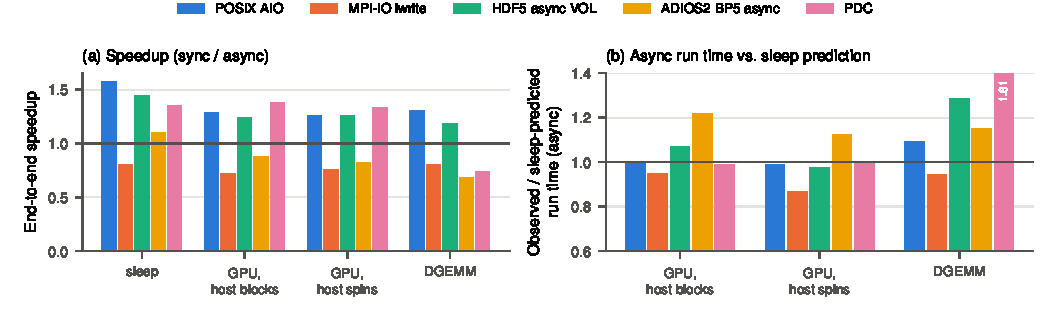
\includegraphics[width=\textwidth]{figures/m_gpu.pdf}
\caption{GPU-resident computation (4 ranks sharing one GPU, 4\,GiB per step,
10 steps). ``Host blocks'' uses blocking synchronization, and ``host spins''
uses the spin-wait of CUDA. DGEMM runs on the CPU with the same 4 ranks.
(a)~End-to-end speedup. (b)~Observed asynchronous run time divided by the
run time that the \texttt{sleep} run predicts.}
\label{fig:gpu}
\end{figure*}

GPU-offloaded codes are where \texttt{sleep} is most often considered
acceptable, because the host is assumed to be idle while the device
computes~\cite{tang2022async}. In Fig.~\ref{fig:gpu}, we test this assumption
with 4 ranks that share the GPU (\srcPhaseGpu, with the wait mode of the host
selected in \srcGpuSetup). Because the GPU idles at a low clock frequency, the
GPU kernels are calibrated at their full length after a warm-up of several
seconds (\srcCalibrate).

Our results largely support the assumption for the asynchronous run.
Fig.~\ref{fig:gpu}b shows that, with a GPU kernel, the asynchronous run time
of POSIX AIO matches the \texttt{sleep} prediction (\GpuexcpctPosixGpuBlock\%
with a blocking host and \GpuexcpctPosixGpuSpin\% with a spinning one), and
HDF5 is within \GpuexcpctHdfGpuBlock\% of it. Non-blocking MPI-IO even runs
faster than predicted. In contrast, the same 4 ranks running DGEMM on the CPU
take \GpuexcpctPosixDgemm\% (POSIX) and \GpuexcpctHdfDgemm\% (HDF5) longer
than the \texttt{sleep} prediction. Whether the host thread blocks or spins
makes little difference in this configuration, because each rank is pinned
to its own core and the background engine shares only the core of its rank.
ADIOS2 is the exception, with run times \GpuexcpctAdiosGpuSpin\% to
\GpuexcpctAdiosGpuBlock\% longer than predicted. However, its compute phase
is short (about 0.7\,s), so this result is the least certain.

However, the end-to-end speedups in Fig.~\ref{fig:gpu}a are still lower with
GPU kernels than with \texttt{sleep}, for example \GpuPosixGpuBlock$\times$
compared to \GpuPosixSleep$\times$ for POSIX and \GpuHdfGpuBlock$\times$
compared to \GpuHdfSleep$\times$ for HDF5. This difference comes from the
synchronous runs. After a \texttt{sleep} phase, the synchronous I/O took
\GpusynciosleepPosix\,s per step for POSIX, compared to
\GpusyncioblockPosix\,s after a GPU kernel, and \GpusynciosleepHdf compared to
\GpusyncioblockHdf\,s for HDF5. This is the same effect we observed in the
main experiment (Section~\ref{sec:threats}). Therefore, for GPU-resident
computation, \texttt{sleep} predicts the asynchronous run time well for most
backends, but it still inflates the speedup by slowing down the synchronous
baseline.

PDC (\srcPhasePdcGpu, with 1 server and 4 clients that share the GPU)
confirms that its interference comes from the CPU. With a GPU kernel, the
asynchronous run time is within \GpuexcpctPdcGpuBlock\% (blocking host) and
\GpuexcpctPdcGpuSpin\% (spinning host) of the \texttt{sleep} prediction, and
the compute phase slows down by only \GpuslowPdcGpuBlock$\times$ and
\GpuslowPdcGpuSpin$\times$. In contrast, the same 4 clients running DGEMM on
the CPU slow down by \GpuslowPdcDgemm$\times$ and take
\GpuexcpctPdcDgemm\% longer than predicted, the largest excess in
Fig.~\ref{fig:gpu}b. For PDC, the speedups with GPU kernels
(\GpuPdcGpuBlock$\times$ and \GpuPdcGpuSpin$\times$) also match the
\texttt{sleep} speedup (\GpuPdcSleep$\times$), unlike for POSIX and HDF5. The
synchronous I/O takes \GpusynciosleepPdc\,s per step after \texttt{sleep}
and \GpusyncioblockPdc\,s after a GPU kernel, so \texttt{sleep} barely
slows down the synchronous baseline of PDC. With DGEMM, the speedup falls to
\GpuPdcDgemm$\times$.

\summarybox{Reserving hardware threads for the background engine recovers
part of the lost benefit for HDF5 and turns non-blocking MPI-IO from a loss
into a small gain, at the cost of fewer compute ranks. For PDC, a reserved
server core is not enough, because the client progress thread competes with
the computation. With GPU-resident
computation and pinned ranks, the host is mostly idle, and \texttt{sleep}
predicts the asynchronous run time within a few percent for POSIX, HDF5,
MPI-IO, and PDC, but not for ADIOS2. The same PDC clients running DGEMM on
the CPU take \GpuexcpctPdcDgemm\% longer than predicted. Even in this case, \texttt{sleep} inflates
the speedup by slowing down the synchronous baseline.}
